\subsection{Implementation of Settings Activity}
\thilemann{Write clever introduction, present the purpose of settings}

\subsubsection{Structure}
\thilemann{How the class is structured, both in xml, i views and in adapters}

\subsubsection{The ''GIRAF'' Pane}
\subsubsection{Launcher Settings}
The settings which are directly in connection with \launcher are presented in \cref{fig:prototypes}.

The available settings are:
\begin{itemize}
 	\item Disabling the start animation, when starting \launcher the first time after a system restart.
 	\item Changing the size of application icons in  \homeactivity.
\end{itemize} 

These are added as suggestions of relevant \launcher settings as outlined in \cref{sec:sprint2:prototypes:settings}.

The most interesting of the two settings is the icon scaling, since ``Show start up animation" is created with a standard Android preference component\footnote{``Preferences'' in Android terminology is what we refer to as ``settings''.}, providing the layout with a two-state switch.

The icon scaling is created by extending the standard \lstinline|Preference| class in Android, thereby inheriting the native setup, i.e. title and summery fields, and constructors for such a component.
We supplement it with a custom layout containing a slider and an application icon, as well as providing functionality to react when the slider changes its position.

\subsubsection{The ''Apps'' Pane}
\subsubsection{Application Settings}
This section follows up from the design described in \cref{sec:sprint3:designsettings}.
When entering the application management fragment, the \lstinline!AppManagementFragment! is loaded into the settings container, seen in \cref{fig:settingsarchitecture} in \lstinline!SettingsActivity!.
The application management fragment in turn contains another fragment container, where the fragments showing the applications are loaded into.
Furthermore, \lstinline!AppContainerFragment! implements three buttons in the top of the layout: the ``Giraf", the ``Android", and the ``Butik" button.\footnote{``Butik'' is Danish for ``store''.}\\

The ``Butik" button opens the  Play Store, so the user can download additional Android applications, if desired. 
We open the Play Store as a separate activity with the \lstinline!Intent.FLAG_ACTIVITY_NEW_TASK! and the \lstinline!Intent.FLAG_ACTIVITY_CLEAR_TOP! flags.
The exact code can be seen in \cref{lst:launchergoogleplay}.\\

The ``Giraf" and the ``Android" buttons load a new fragment into  \lstinline!AppsContainer!, by using a \lstinline!FragmentManager! - the same way it is described in \cref{sec:settingslistfragment}.\\

The fragments loaded are derived from the same superclass, called \lstinline|AppContainerFragment| and is described subsequently.
%An  \lstinline!OnClickListener! is attached to the \textbf{Giraf} and \textbf{Android} buttons, which call the method \lstinline!replaceFragment()!, sending the appropriate fragment as argument to \lstinline!replaceFragment()!.
%The method \lstinline!replaceFragment()! can be seen in \cref{lst:replaceFragment}.
%
%\begin{lstlisting}[caption={Method used to replace the fragment currently loaded into the fragment container in AppManagementFragment}, label={lst:replaceFragment}]
%/**
% * Replace active fragment by running the transaction in a new thread.
% * Adds responsiveness when loading list of installed apps_container.
% * @param fragment
% */
%private void replaceFragment(final Fragment fragment){
%    new Runnable() {
%        @Override
%        public void run() {
%            FragmentTransaction ft = fragmentManager.beginTransaction();
%            ft.replace(R.id.app_settings_fragmentlayout, fragment);
%            ft.commit();
%        }
%    }.run();
%}
%\end{lstlisting}

%Firstly, we researched how to use the inbuilt API for Google Services  to open the Play Store in this way.
%However, there were some problems with the API when attempting to implement.
%Furthermore, it was discovered that the API is intended to be used for syncronization with Google+, Google Drive and Google Games.


%The full design can be seen visualized in \cref{fig:settingsappfragments}.
 
%\begin{figure}[h]
%\centering
%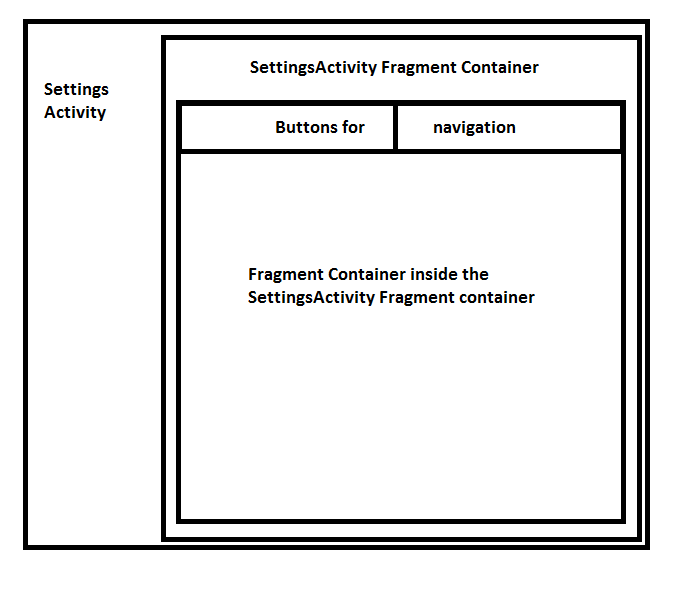
\includegraphics[width=\textwidth, height=3in, keepaspectratio=true] {SettingsActivity.png}
%\caption{The organization of \lstinline!SettingsActivity! when inside the "Apps" pane. Since we need to distinguish between \giraf and Android applications, nested fragment containers are used.}
%\label{fig:settingsappfragments}
%\end{figure}

\subsubsection{AppContainerFragment and the derived classes}

Because the \giraf and Android fragments contain many of the same variables, these inherit all shared information from a superclass, consequently reducing redundancy and clarifying how the two fragments are different.
This superclass is called \lstinline!AppManagementFragment! and the main responsibilities are:

\begin{itemize}
\item Initialize shared variable in \lstinline!onCreate()!
\item Implement shared methods handling when to load applications
\end{itemize}

As a result, the two derived classes get their shared variables initialized by a call to \lstinline!super.onCreate()! and reloading of applications is handled automatically by \lstinline!AppContainerFragment!. \\

However, which type of applications are loaded is different for \lstinline!AndroidFragment! and \lstinline!GirafFragment!.
%As noted in \cref{sec:sprint:designlauncher} and explained in \cref{sect:sprint3:refactoring}, the functions used to load applications into view was moved from \lstinline!HomeActivity! to \lstinline!LauncherUtility!.
This is solved by initializing the shared variable \lstinline!apps! differently in the two derived classes -
\lstinline!GirafFragment! loads \giraf applications into \lstinline!apps!, while \lstinline!AndroidFragment! loads Android applications into it.

Since the automatic load methods mentioned above work on the \lstinline!apps! variable, this solution solves the problem. \\

The other problem present is related to the marking of applications.
%However, one problem has to be directly inside the two derived classes, namely marking the applications as selected and adding them to the users list of selected applications.
This is due to the fact that \giraf applications are saved as the \textit{OasisLib} type \lstinline!Application!, while Android applications are saved as the type \lstinline!ResolveInfo!.

The \giraf applications connected to a user are saved or removed through a call to an \textit{OasisLib} method, while Android applications are saved as a file stored in the native \lstinline!SharedPreferences! of Android.
%Each file name is made, unique to each user, by incorporating the users ID as part of the file name.
More about saving settings in Android can be found in \cref{para:sprint4:managingsettingsandroid} and the code for marking the applications can be seen in \cref{lappendix:markingapps}\\

%This also means that the two fragments must handle the selected applications different, when marking them the first time a fragment is loaded.
%The code is not included, since it is similar to that of \cref{lst:addinggirafapplications} and \cref{lst:addingandroidapplications} - the same checks are carried out, but rather than being for a single application, they are carried out on all installed applications.

These two problems are the main reason we need to derive the two subclasses.\\

Having described all the different types of settings \launcher treats, the next sections explains how to save the settings.

 \subsubsection{The ''Android Settings'' Pane}
 * | f4346e2 (2 weeks ago) thilemann@gmail.com Added button to access Android Settings from giraf settings app and cleaned up the onclicklistener for google play button and removed bold fontface from tab buttons when active\\
 
 \subsubsection{Starting settings of other apps from Settings}
 * | | c51e137 (7 days ago) thilemann@gmail.com Cleaned file and removed unnecessary intent-filter from SettingsActivity. This activity should not be available through an intent.
 * | bd0c2c7 (7 days ago) thilemann@gmail.com When adding an intent by packagename there were no checks that the intent indeed contains the action needed to start the settings of the application. This is now
 handled so it is not added to the list if it does not exist.
 * | | | 6f19b2e (7 days ago) thilemann@gmail.com Added Sequence (Zebra) to settings
 | * | | 0bb96b3 (7 days ago) jesper.b.kjaer@gmail.com Added handling of ActivityNotFound exception in settings.